\documentclass{article}

\usepackage{subcaption}

\usepackage{graphicx}
\usepackage{wrapfig}
\usepackage{picinpar}
\usepackage{cutwin}

\begin{document}

\section{wrapfig}

\begin{wrapfigure}{l}[1cm]{0pt}
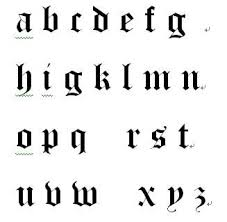
\includegraphics[width=2.5cm]{figures/abc.jpeg}
\caption{Podala Palace, Tibet}label{fig:tibet}
\end{wrapfigure}
text text text text text text text text
text text text text text text text text
text text text text text text text text 
text text text text text text text text
text text text text text text text text
text text text text text text text text
text text text text text text text text
text text text text text text text text
text text text text text text text text
text text text text text text text text
text text text text text text text text
text text text text text text text text
text text text text text text text text
text text text text text text text text
text text text text text text text text
text text text text text text text text
text text text text text text text text
text text text text text text text text
text text text text text text text text
text text text text text text text text
text text text text text text text text
text text text text text text text text


% https://www.zhihu.com/question/26837705
\section{picinpar}%对插入图表位置有特殊要求,用picinpar

\begin{figwindow}[2,c,
   {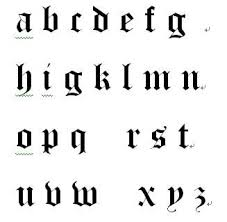
\includegraphics[width=2.5cm]{figures/abc.jpeg}},
   picinpar]
text text text text text text text text
text text text text text text text text
text text text text text text text text 
text text text text text text text text
text text text text text text text text
text text text text text text text text
text text text text text text text text
text text text text text text text text
text text text text text text text text
text text text text text text text text
text text text text text text text text
text text text text text text text text
text text text text text text text text
\end{figwindow}

\section{cutwin}%对位置或形状有较高要求,用cutwin

\renewcommand{\windowpagestuff}{%
    \quad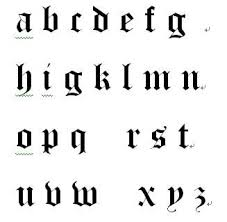
\includegraphics[width=2.5cm]{figures/abc.jpeg}}
\begin{cutout}{2}{2.2cm}{6.2cm}{6}
 text text text text text text text text
 text text text text text text text text
 text text text text text text text text 
 text text text text text text text text
 text text text text text text text text
 text text text text text text text text
 text text text text text text text text
 text text text text text text text text
 text text text text text text text text
 text text text text text text text text
 text text text text text text text text
 text text text text text text text text
 text text text text text text text text
 \end{cutout}


\begin{figure*}
    \centering
    \begin{subfigure}[b]{0.22\textwidth}
        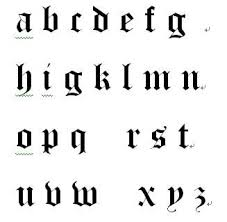
\includegraphics[width=2.5cm]{figures/abc.jpeg}
        \caption{Input Image}
        \label{fig:visual_smap_o}
    \end{subfigure}
    \begin{subfigure}[b]{0.22\textwidth }
        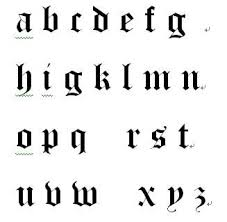
\includegraphics[width=2.5cm]{figures/abc.jpeg}
        \caption{Original }
        \label{fig:visual_smap_k}
    \end{subfigure}
    \begin{subfigure}[b]{0.22\textwidth }%0.22表示图片间的间隔;
        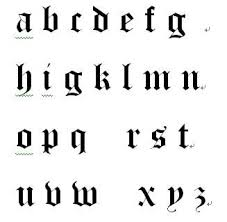
\includegraphics[width=2.5cm]{figures/abc.jpeg}
        \caption{Enhanced }%文字描述部分;
        \label{fig:visual_smap_c}%\label{fig:visual_smap_gt},可用可无,用来标记这张图片,后面可以用来索引。
    \end{subfigure}
    \begin{subfigure}[b]{0.22\textwidth}
        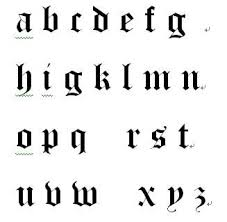
\includegraphics[width=2.5cm]{figures/abc.jpeg}
        \caption{Ground }
        \label{fig:visual_smap_gt}
    \end{subfigure}
    \caption{Visual comparison samples between the original saliency map and enhanced saliency map by centre-bias and human visual acuity.}
\label{fig:visual_smap}
\end{figure*}

\end{document}




在使用 wrapfig 时需要注意下面几点:

    - 在 wrapfigure 后必须紧接着输入段落文字,否则会出错。
    - 不能在任何列表环境中使用 wrapfigure,也不能在 列表环境前后使用,除非两者之间有一空行或分段指令 \par。
    - 如果将 wrapfigure 放在 \parbox 或小页环境 等分组中,文本折行必须在这些分组前结束。
    - 在双栏页版式中不能使用 wrapfigure。
    - 如果在 wrapfigure 中使用 figure 等 浮动对象,它的编号有可能不正确。
    - 如果在 wrapfigure 中使用 table 等浮动对象, 它上下方的横线可能被忽略,必须自己再加入。
    - 在折行的文本中, \linewidth 并没有改变。

    begin{wrapfigure}{行数}[位置][超出长度]{宽度}<图形>end{wrapfigure}

    \begin{wrapfigure}{l}[1cm]{0pt}
        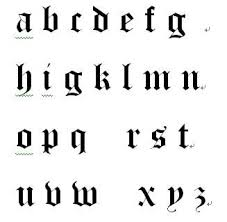
\includegraphics[width=2.5cm]{figures/abc.jpeg}
        \caption{Podala Palace, Tibet}label{fig:tibet}
        \end{wrapfigure}

    - 这里行数是指图形高度所占的文本行的数目。如果不给出此选项,wrapfig会自动计算。
    - 位置是指图形相对于文本的位置,须给定下面四项的一个。
        - [r],[R]:表示图形位于文本的左边。
        - [l],[L]:表示图形位于文本的右边。
        - [i],[R]: 表示图形位于页面靠里的一边(用在双面格式里)。
        - [o],[O]: 表示图形位于页面靠外的一边。
    - 超出长度是指图形超出文本边界的长度,缺省为 0pt。
    - 宽度则指图形的宽度。wrapfig会自动计算图形的高度。

